\subsection{UC26 - Modifica informazioni utente}\label{usecase:26}
\begin{figure}[H]
\centering
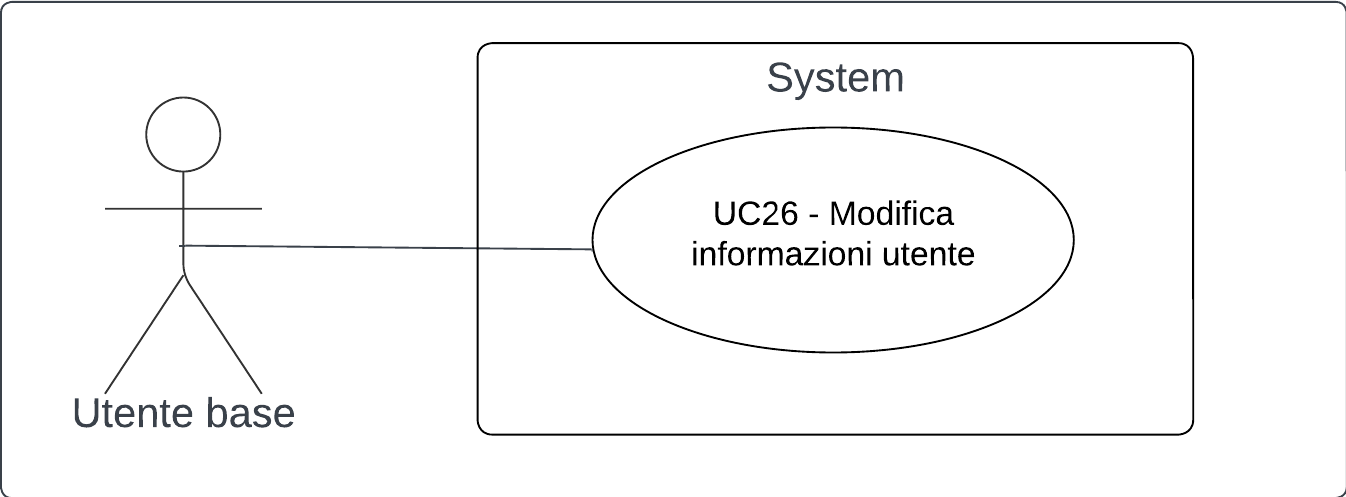
\includegraphics[width=0.75\linewidth]{ucd/UCD26}
\end{figure}
\textbf{Attori}:
\begin{itemize}
    \item Utente base
\end{itemize}
\textbf{Precondizioni}:
\begin{itemize}
    \item L'utente deve essere autenticato
\end{itemize}
\textbf{Postcondizioni}:
\begin{itemize}
    \item L'utente ha inserito le informazioni
\end{itemize}
\textbf{\textit{Scenario}_G principale}:
\begin{enumerate}
    \item L'utente inserisce il suo nome
    \item L'utente inserisce il suo cognome
    \item L'utente inserisce un email valida
    \item l'utente inserisce la sua password
\end{enumerate}
\textbf{Scenari alternativi}:
\begin{enumerate}
    \item Nel caso in cui l'email sia già presente all'interno del sistema, l'utente viene notificato attraverso un messaggio visivo.
    \item Viene data la possibilità all'utente di scegliere un'email valida.
\end{enumerate}
\newpage